\documentclass[aspectratio=43]{beamer}

% Title --------------------------------------------
\title{\huge Transitional Justice\\\vspace{5pt}and Human Rights}
\author{Francisco Villamil}
\date{War, peace, and political violence\\UC3M, Fall 2023}

%%% NOTE -- CHECK THIS: https://github.com/paulgp/beamer-tips


%%% Building heavily on https://github.com/kylebutts/templates

% xcolor, define them
\usepackage{xcolor}

% TEXT COLORS
\definecolor{red}{HTML}{9a2515}
\definecolor{yellow}{HTML}{EBC944}
\definecolor{asher}{HTML}{555F61}
\definecolor{jet}{HTML}{131516}

% THEME COLORS
\definecolor{accent}{HTML}{107895}
\definecolor{accent2}{HTML}{9a2515}

% Color commands
\newcommand\red[1]{{\color{red}#1}}
\newcommand\yellow[1]{{\color{yellow}#1}}
\newcommand\asher[1]{{\color{asher}#1}}

\newcommand\BGred[1]{{\colorbox{red!80!white}{#1}}}
\newcommand\BGyellow[1]{{\colorbox{yellow!80!white}{#1}}}
\newcommand\BGasher[1]{{\colorbox{asher!80!white}{#1}}}

\renewcommand<>{\BGyellow}[1]{\only#2{\beameroriginal{\BGyellow}}{#1}}

% Appendix numbering
\usepackage{appendixnumberbeamer}

% Beamer Options -------------------------------------

% Background
\setbeamercolor{background canvas}{bg = white}

% Change text margins
\setbeamersize{text margin left = 25pt, text margin right = 15pt}

% \alert
\setbeamercolor{alerted text}{fg = accent2}

% Frame title
\setbeamercolor{frametitle}{bg = white, fg = jet}
\setbeamercolor{framesubtitle}{bg = white, fg = accent}
\setbeamerfont{framesubtitle}{size = \small, shape = \itshape}

% Block
\setbeamercolor{block title}{fg = white, bg = accent2}
\setbeamercolor{block body}{fg = jet, bg = jet!10!white}

% Title page
\setbeamercolor{title}{fg = jet}
\setbeamercolor{subtitle}{fg = accent}

%% Custom \maketitle and \titlepage
\setbeamertemplate{title page}
{
    \begin{centering}
      % \vspace{20mm}
      {\Large \usebeamerfont{title}\usebeamercolor[fg]{title}\inserttitle}\\ \vskip0.25em%
      \ifx\insertsubtitle\@empty%
      \else%
        {\usebeamerfont{subtitle}\usebeamercolor[fg]{subtitle}\insertsubtitle\par}%
      \fi%
      {\vspace{10mm}\insertauthor}\\
      \ifx\insertinstitute\@empty%
      \else%
        {\vspace{5mm}\color{asher}\scriptsize{\insertinstitute}}
      \fi%
      {\color{asher}\small{\insertdate}}\\
    \end{centering}
}

% Table of Contents
\setbeamercolor{section in toc}{fg = accent!70!jet}
\setbeamercolor{subsection in toc}{fg = jet}

% Button
\setbeamercolor{button}{bg = accent}

% Remove navigation symbols
\setbeamertemplate{navigation symbols}{}

% Table and Figure captions
\setbeamercolor{caption}{fg=jet!70!white}
\setbeamercolor{caption name}{fg=jet}
\setbeamerfont{caption name}{shape = \itshape}

% Put slide number / total slides at the bottom right
\makeatother
\makeatletter
\setbeamertemplate{footline} %{\hfill\insertframenumber/\inserttotalframenumber}
{%
  \leavevmode%
  \hbox{
  \begin{beamercolorbox}[wd=\paperwidth,ht=2.5ex,dp=1.125ex,leftskip=.3cm,rightskip=.3cm plus1fil]{footlinecolor}%
    \color{asher}{\hfill\insertframenumber/\inserttotalframenumber}
  \end{beamercolorbox}}%
  \vskip0pt%
}
\makeatother
\makeatletter

% Bullet points

%% Fix left-margins
\settowidth{\leftmargini}{\usebeamertemplate{itemize item}}
\addtolength{\leftmargini}{\labelsep}

%% enumerate item color
\setbeamercolor{enumerate item}{fg = accent}
\setbeamerfont{enumerate item}{size = \small}
\setbeamertemplate{enumerate item}{\insertenumlabel.}

%% itemize
\setbeamercolor{itemize item}{fg = accent!70!white}
\setbeamerfont{itemize item}{size = \small}
\setbeamertemplate{itemize item}[circle]
\setlength{\itemsep}{0pt plus 6pt}

%% right arrow for subitems
\setbeamercolor{itemize subitem}{fg = accent!60!white}
\setbeamerfont{itemize subitem}{size = \small}
\setbeamertemplate{itemize subitem}{$\rightarrow$}

\setbeamertemplate{itemize subsubitem}[square]
\setbeamercolor{itemize subsubitem}{fg = jet}
\setbeamerfont{itemize subsubitem}{size = \small}

% References

%% Bibliography Font, roughly matching aea
\setbeamerfont{bibliography item}{size = \footnotesize}
\setbeamerfont{bibliography entry author}{size = \footnotesize, series = \bfseries}
\setbeamerfont{bibliography entry title}{size = \footnotesize}
\setbeamerfont{bibliography entry location}{size = \footnotesize, shape = \itshape}
\setbeamerfont{bibliography entry note}{size = \footnotesize}

\setbeamercolor{bibliography item}{fg = jet}
\setbeamercolor{bibliography entry author}{fg = accent!60!jet}
\setbeamercolor{bibliography entry title}{fg = jet}
\setbeamercolor{bibliography entry location}{fg = jet}
\setbeamercolor{bibliography entry note}{fg = jet}

%% Remove bibliography symbol in slides
\setbeamertemplate{bibliography item}{}





% Links ----------------------------------------------

\usepackage{hyperref}
\hypersetup{
  colorlinks = true,
  linkcolor = accent,
  filecolor = accent,
  urlcolor = accent,
  citecolor = accent,
}


% Line spacing --------------------------------------
\usepackage{setspace}
\setstretch{1.2}


% \begin{columns} -----------------------------------
\usepackage{multicol}


% % Fonts ---------------------------------------------
% % Beamer Option to use custom fonts
% \usefonttheme{professionalfonts}
%
% % \usepackage[utopia, smallerops, varg]{newtxmath}
% % \usepackage{utopia}
% \usepackage[sfdefault,light]{roboto}
%
% % Small adjustments to text kerning
% \usepackage{microtype}



% Remove annoying over-full box warnings -----------
\vfuzz2pt
\hfuzz2pt


% Table of Contents with Sections
\setbeamerfont{myTOC}{series=\bfseries, size=\Large}
\AtBeginSection[]{
        \frame{
            \frametitle{Roadmap}
            \tableofcontents[current]
        }
    }


% References ----------------------------------------
\usepackage[
    citestyle= authoryear,
    style = authoryear,
    natbib = true,
    backend = biber
]{biblatex}

% Smaller font-size for references
\renewcommand*{\bibfont}{\small}

% Remove "In:"
\renewbibmacro{in:}{}

% Color citations for slides
\newenvironment{citecolor}
    {\footnotesize\begin{color}{accent2}}
    {\end{color}}

\newcommand{\citetcolor}[1]{{\footnotesize\textcolor{asher}{\citet{#1}}}}
\newcommand{\citepcolor}[1]{{\footnotesize\textcolor{asher}{\citep{#1}}}}

% Tables -------------------------------------------
% Tables too big
% \begin{adjustbox}{width = 1.2\textwidth, center}
\usepackage{adjustbox}
\usepackage{array}
\usepackage{threeparttable, booktabs, adjustbox}

% Fix \input with tables
% \input fails when \\ is at end of external .tex file

\makeatletter
\let\input\@@input
\makeatother

% Tables too narrow
% \begin{tabularx}{\linewidth}{cols}
% col-types: X - center, L - left, R -right
% Relative scale: >{\hsize=.8\hsize}X/L/R
\usepackage{tabularx}
\newcolumntype{L}{>{\raggedright\arraybackslash}X}
\newcolumntype{R}{>{\raggedleft\arraybackslash}X}
\newcolumntype{C}{>{\centering\arraybackslash}X}

% Figures

% \imageframe{img_name} -----------------------------
% from https://github.com/mattjetwell/cousteau
\newcommand{\imageframe}[1]{%
    \begin{frame}[plain]
        \begin{tikzpicture}[remember picture, overlay]
            \node[at = (current page.center), xshift = 0cm] (cover) {%
                \includegraphics[keepaspectratio, width=\paperwidth, height=\paperheight]{#1}
            };
        \end{tikzpicture}
    \end{frame}%
}

% subfigures
\usepackage{subfigure}


% Highlight slide -----------------------------------
% \begin{transitionframe} Text \end{transitionframe}
% from paulgp's beamer tips
\newenvironment{transitionframe}{
    \setbeamercolor{background canvas}{bg=accent!60!black}
    \begin{frame}\color{accent!10!white}\LARGE\centering
}{
    \end{frame}
}


% Table Highlighting --------------------------------
% Create top-left and bottom-right markets in tabular cells with a unique matching id and these commands will outline those cells
\usepackage[beamer,customcolors]{hf-tikz}
\usetikzlibrary{calc}
\usetikzlibrary{fit,shapes.misc}

% To set the hypothesis highlighting boxes red.
\newcommand\marktopleft[1]{%
    \tikz[overlay,remember picture]
        \node (marker-#1-a) at (0,1.5ex) {};%
}
\newcommand\markbottomright[1]{%
    \tikz[overlay,remember picture]
        \node (marker-#1-b) at (0,0) {};%
    \tikz[accent!80!jet, ultra thick, overlay, remember picture, inner sep=4pt]
        \node[draw, rectangle, fit=(marker-#1-a.center) (marker-#1-b.center)] {};%
}



\begin{document}

\begin{frame}
  \titlepage
\end{frame}

% ----------------------------------------------------
\imageframe{img/WarOver-newspaper}
% ----------------------------------------------------

% ----------------------------------------------------
\begin{frame}
\frametitle{Transitional Justice}
\centering

\begin{itemize}
  \item \BGyellow{Transitional Justice} is a set of policies employed in the aftermath of war or regime change (democratization)
\end{itemize}

\end{frame}
% ----------------------------------------------------

% ----------------------------------------------------
\begin{frame}<1>[label=tj_types]
\frametitle{Mechanisms of TJ}
\centering

\begin{itemize}
  \item \BGyellow<1>{Criminal trials}
  \begin{itemize}
    \item<2-> vs. \BGyellow<2>{Amnesties}: we might not see it as a `TJ mechanism', but state leaders usually do
  \end{itemize}
  \item<3-> \BGyellow<3>{Reparations}
  \item<4-> \BGyellow<4>{Lustration}
  \item<5-> \BGyellow<5>{Truth}
  \item<6-> \BGyellow<6>{Memory \& symbols}
  \item<7-> \BGyellow<7>{Others:}
  \begin{itemize}
    \item Institutional reform, gender-specific TJ, ...
  \end{itemize}
\end{itemize}

\end{frame}
% ----------------------------------------------------

% ----------------------------------------------------
\imageframe{img/nuremberg}
% ----------------------------------------------------

% ----------------------------------------------------
\begin{frame}
\frametitle{Nüremberg Trials}
\centering

\begin{itemize}
  \item First \textit{international war crimes} tribunal in history
  \item<2-> New ideas: crimes against humanity, crimes against peace
  \begin{itemize}
    \item Different from old \textit{jus in bello}
  \end{itemize}
  \item<3-> Importance of the Holocaust
  \item<4-> Context: interstate war, military defeat
\end{itemize}

\end{frame}
% ----------------------------------------------------

% ----------------------------------------------------
\begin{frame}
\frametitle{Tokyo Trials}
\centering

\begin{minipage}{0.49\textwidth}\centering
\only<2>{\begin{itemize}
  \linespread{0.9}\selectfont
  \item Same as Nüremberg?
  \item The case of Kōki Hirota
  \item[] {\small (only civilian sentenced to death)}
  \item[]
  \item[-] {\footnotesize \href{https://www.newyorker.com/magazine/2023/10/23/judgment-at-tokyo-world-war-ii-on-trial-and-the-making-of-modern-asia-gary-j-bass-book-review}{`What the Tokyo Trial Reveals About Empire, Memory, and Judgment'}}
\end{itemize}}
\end{minipage}\hfill
\begin{minipage}{0.5\textwidth}\centering
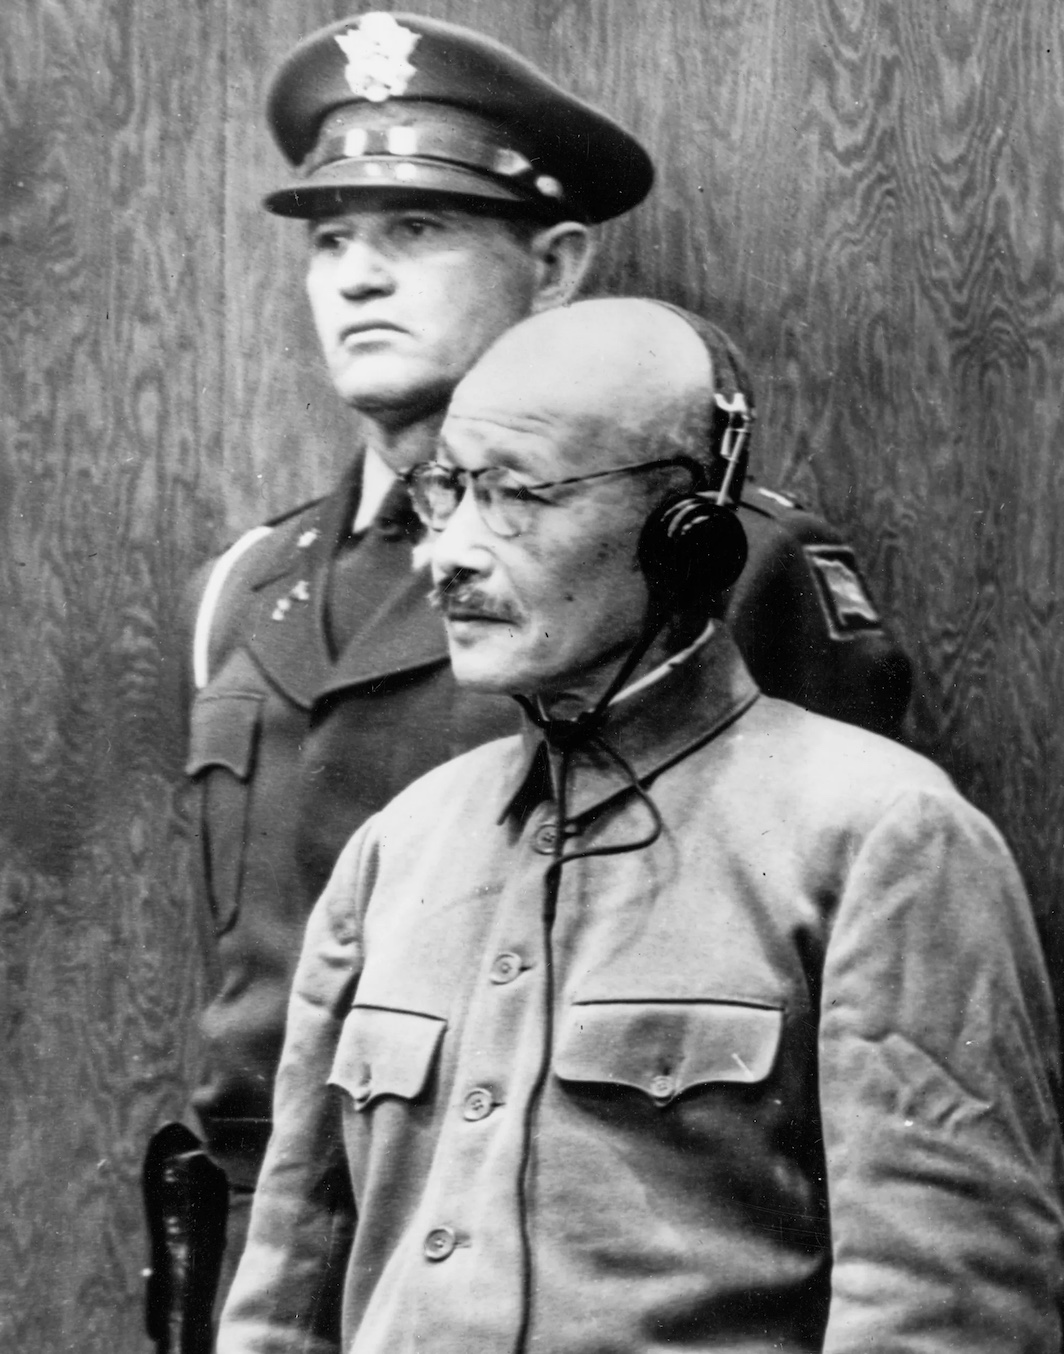
\includegraphics[width = .75\textwidth]{img/tojo}\\
Hideki Tojo, 1948
\end{minipage}

\end{frame}
% ----------------------------------------------------

% ----------------------------------------------------
\imageframe{img/milosevic}
% ----------------------------------------------------

% ----------------------------------------------------
\begin{frame}
\frametitle{ICTY}
\centering

\begin{minipage}{.49\textwidth}\centering
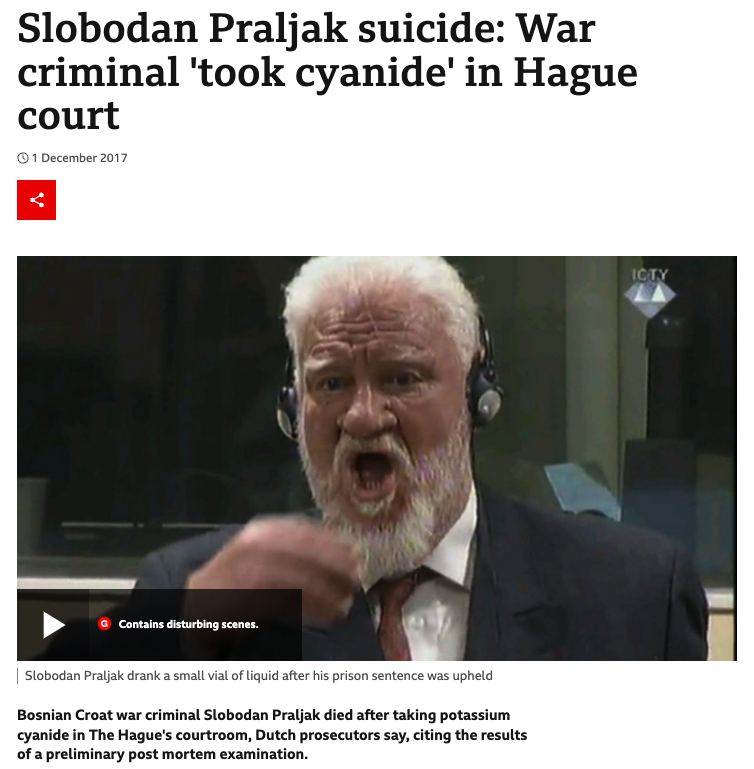
\includegraphics[width = \textwidth]{img/praljak}
\end{minipage}\hfill
\begin{minipage}{.49\textwidth}\centering
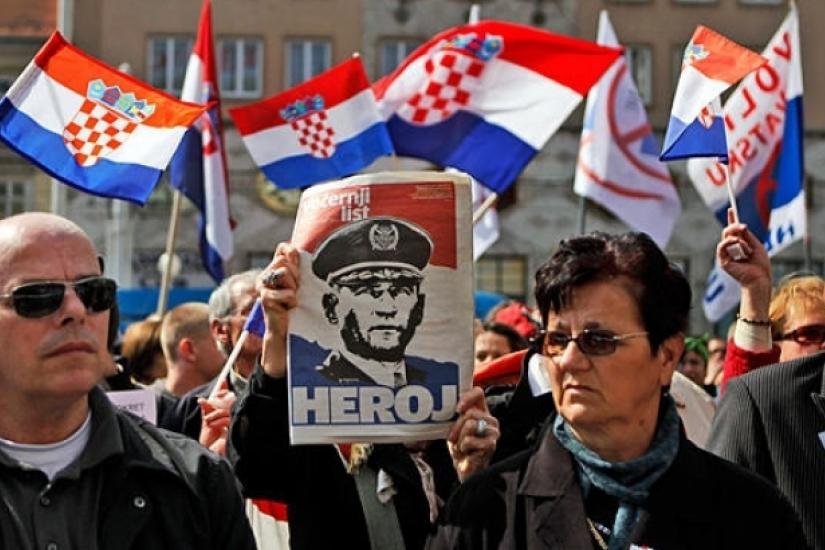
\includegraphics[width = \textwidth]{img/gotovina}\\{\small Ante Gotovina trial}
\end{minipage}

\end{frame}
% ----------------------------------------------------

% ----------------------------------------------------
\imageframe{img/juicio_juntas}
% ----------------------------------------------------

% % ----------------------------------------------------
% \imageframe{img/argentina1985}
% % ----------------------------------------------------

% ----------------------------------------------------
\begin{frame}
\frametitle{}
\centering

\begin{minipage}{0.4\textwidth}\centering
\only<2->{\begin{itemize}
  \item \BGyellow{Trial of the Juntas}
  \item Early example of \textit{domestic} human rights prosecution
  \begin{itemize}
    \item<2-> Not the first though (Greek junta trials, Portugal (limited) trials)
  \end{itemize}
  \item<3-> A third option are \textit{foreign trials}
\end{itemize}}
\end{minipage}\hfill
\begin{minipage}{0.59\textwidth}\centering
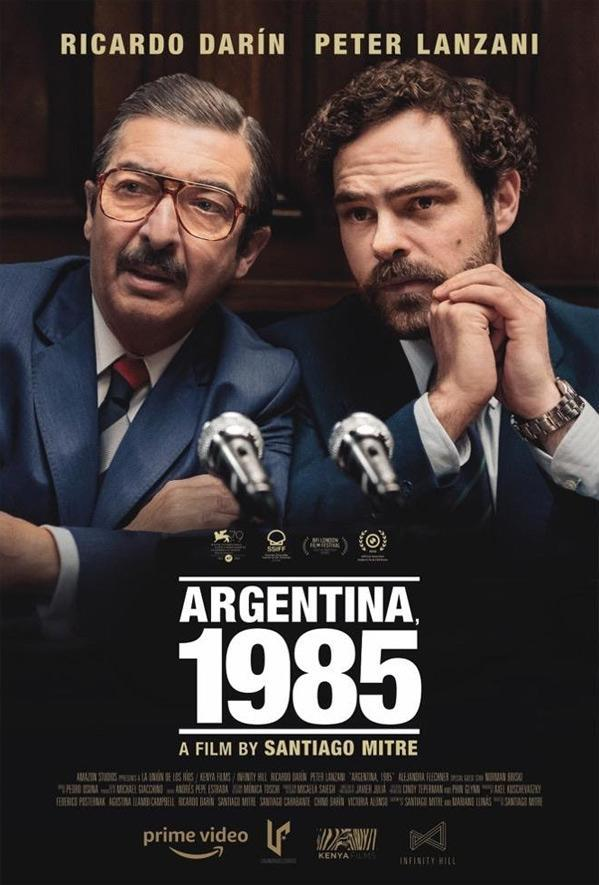
\includegraphics[width = 0.9\textwidth]{img/argentina1985b}
\end{minipage}

\end{frame}
% ----------------------------------------------------

% ----------------------------------------------------
\imageframe{img/pinochet}
% ----------------------------------------------------

% ----------------------------------------------------
\againframe<1-3>{tj_types}
% ----------------------------------------------------

% ----------------------------------------------------
\begin{frame}
\frametitle{}
\centering


\includegraphics[width = \textwidth]{img/udhr}\\

\includegraphics[width = \textwidth]{img/udhr2}

\end{frame}
% ----------------------------------------------------

% ----------------------------------------------------
\imageframe{img/reparations_US}
% ----------------------------------------------------

% ----------------------------------------------------
\againframe<4>{tj_types}
% ----------------------------------------------------

% ----------------------------------------------------
\imageframe{img/lustration_poland}
% ----------------------------------------------------

% ----------------------------------------------------
\begin{frame}
\frametitle{Lustrations}
\centering

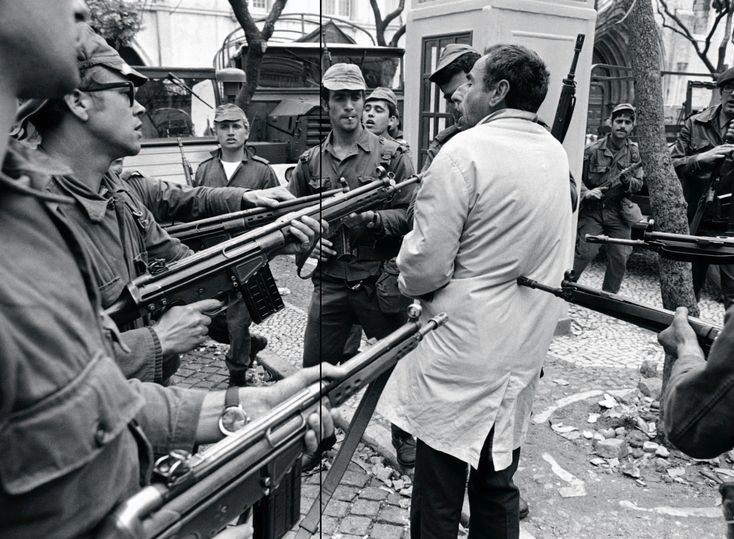
\includegraphics[width = \textwidth]{img/pide}

Suspected PIDE member in Lisbon, April 25th, 1974

\end{frame}
% ----------------------------------------------------

% ----------------------------------------------------
\imageframe{img/depuracion_magisterio}
% ----------------------------------------------------

% ----------------------------------------------------
\imageframe{img/mccarthy}
% ----------------------------------------------------

% ----------------------------------------------------
\againframe<5>{tj_types}
% ----------------------------------------------------

% ----------------------------------------------------
\begin{frame}
\frametitle{}
\centering

\begin{minipage}{.49\textwidth}\centering
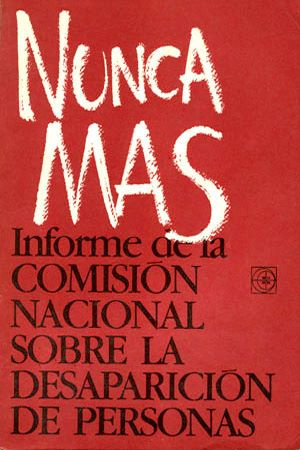
\includegraphics[width = \textwidth]{img/argentina_nuncamas}\\Argentina (1984)
\end{minipage}\hfill
\begin{minipage}{.49\textwidth}\centering
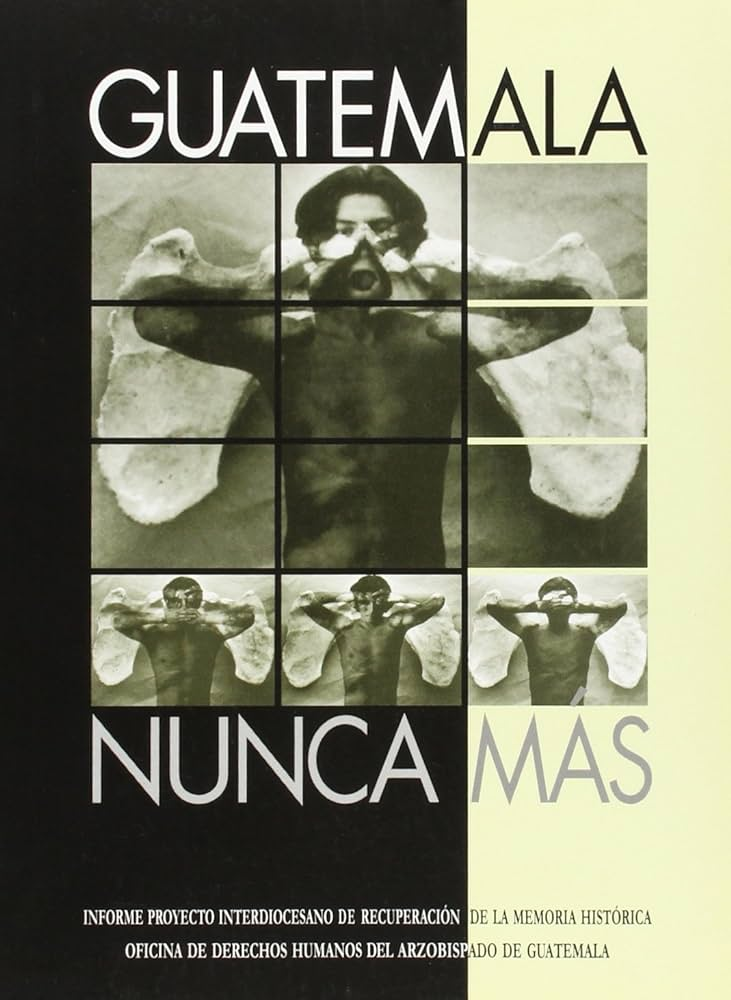
\includegraphics[width = \textwidth]{img/guatemala_nuncamas}\\Guatemala (1998)
\end{minipage}

\end{frame}
% ----------------------------------------------------

% ----------------------------------------------------
\imageframe{img/trc_zaf}
% ----------------------------------------------------

% ----------------------------------------------------
\imageframe{img/gogora}
% ----------------------------------------------------

% ----------------------------------------------------
\imageframe{img/portalvictimas}
% ----------------------------------------------------

% ----------------------------------------------------
\imageframe{img/fosas}
% ----------------------------------------------------

% ----------------------------------------------------
\againframe<6>{tj_types}
% ----------------------------------------------------

% ----------------------------------------------------
\imageframe{img/franco_calles}
% ----------------------------------------------------

% ----------------------------------------------------
\imageframe{img/denizafication}
% ----------------------------------------------------

% ----------------------------------------------------
\imageframe{img/leninopad}
% ----------------------------------------------------

% ----------------------------------------------------
\imageframe{img/franco_exhumation}
% ----------------------------------------------------

% ----------------------------------------------------
\againframe<7->{tj_types}
% ----------------------------------------------------

% ----------------------------------------------------
\imageframe{img/countries_by_year.pdf}
% ----------------------------------------------------

% ----------------------------------------------------
\begin{frame}
\frametitle{}
\centering

\begin{itemize}
  \item What do you think are the goals of TJ?
\end{itemize}

\end{frame}
% ----------------------------------------------------

% ----------------------------------------------------
\begin{frame}<1>[label=tj_q]
\frametitle{Questions}
\centering

\begin{itemize}
  \item The causes of TJ policies
  \begin{itemize}
    \item<2-> emergence of human rights \textit{norms}: how and why?
    \item<3-> determinants of domestic policies: what explains that some countries apply them?
    \item<4-> role of international factors in explaining TJ difussion?
  \end{itemize}
  \item<5-> \BGyellow<5->{The consequences}
  \begin{itemize}
    \item<6-> what are the consequences at the elite-level?
    \item<7-> do they have an effect beyond one particular country?
    \item<8-> effects at the \textit{micro}-level? (reconciliation, etc)
  \end{itemize}

\end{itemize}

\end{frame}
% ----------------------------------------------------

% ----------------------------------------------------
\begin{frame}
\frametitle{TJ and human rights}
\centering

\begin{itemize}
  \item Why do we observe Transitional Justice policies?
  \begin{itemize}
    \item especially, why do we observe \textit{domestic} prosecutions?
  \end{itemize}
  \item This is a debate related to the emergence of \BGyellow{human rights}
\end{itemize}

\end{frame}
% ----------------------------------------------------

% ----------------------------------------------------
\begin{frame}
\frametitle{How did human rights develop?}
\centering

\begin{itemize}
  \item We live in a world where human rights are the \BGyellow{norm}
  \item<2-> But it was not always like that
  \begin{itemize}
    \item<3-> School of Salamanca and natural law
    \item<4-> Enlightment and Reformation
    \item<5-> Post-WWII
  \end{itemize}
  \item<6-> \textbf{How and why did we get here?}
  \begin{itemize}
    \item What is the process that explains the expansion of human rights norms and institutions to enforce them, both at the domestic and international level?
    \item<6-> Why this is important: can we actually \textit{promote} human rights?
  \end{itemize}
\end{itemize}


\end{frame}
% ----------------------------------------------------

% ----------------------------------------------------
\begin{frame}
\frametitle{Power leads, rights follow}
\centering

\begin{minipage}{.59\textwidth}\centering

\begin{itemize}
  \item Human rights are all about \BGyellow{liberal modernity}
  \item<2-> Only when \textbf{middle classes} emerge and become strong, forming \textbf{winning coalitions}
  \begin{itemize}
    \item Historical role of the emergence of a trading class in Northern Europe and Protestant Reformation
    \item Setbacks during the 20th Century
  \end{itemize}
  \item<3-> \textbf{Liberal} and \textbf{realist} theories of HR?
\end{itemize}

\end{minipage}\hfill
\begin{minipage}{.40\textwidth}\centering
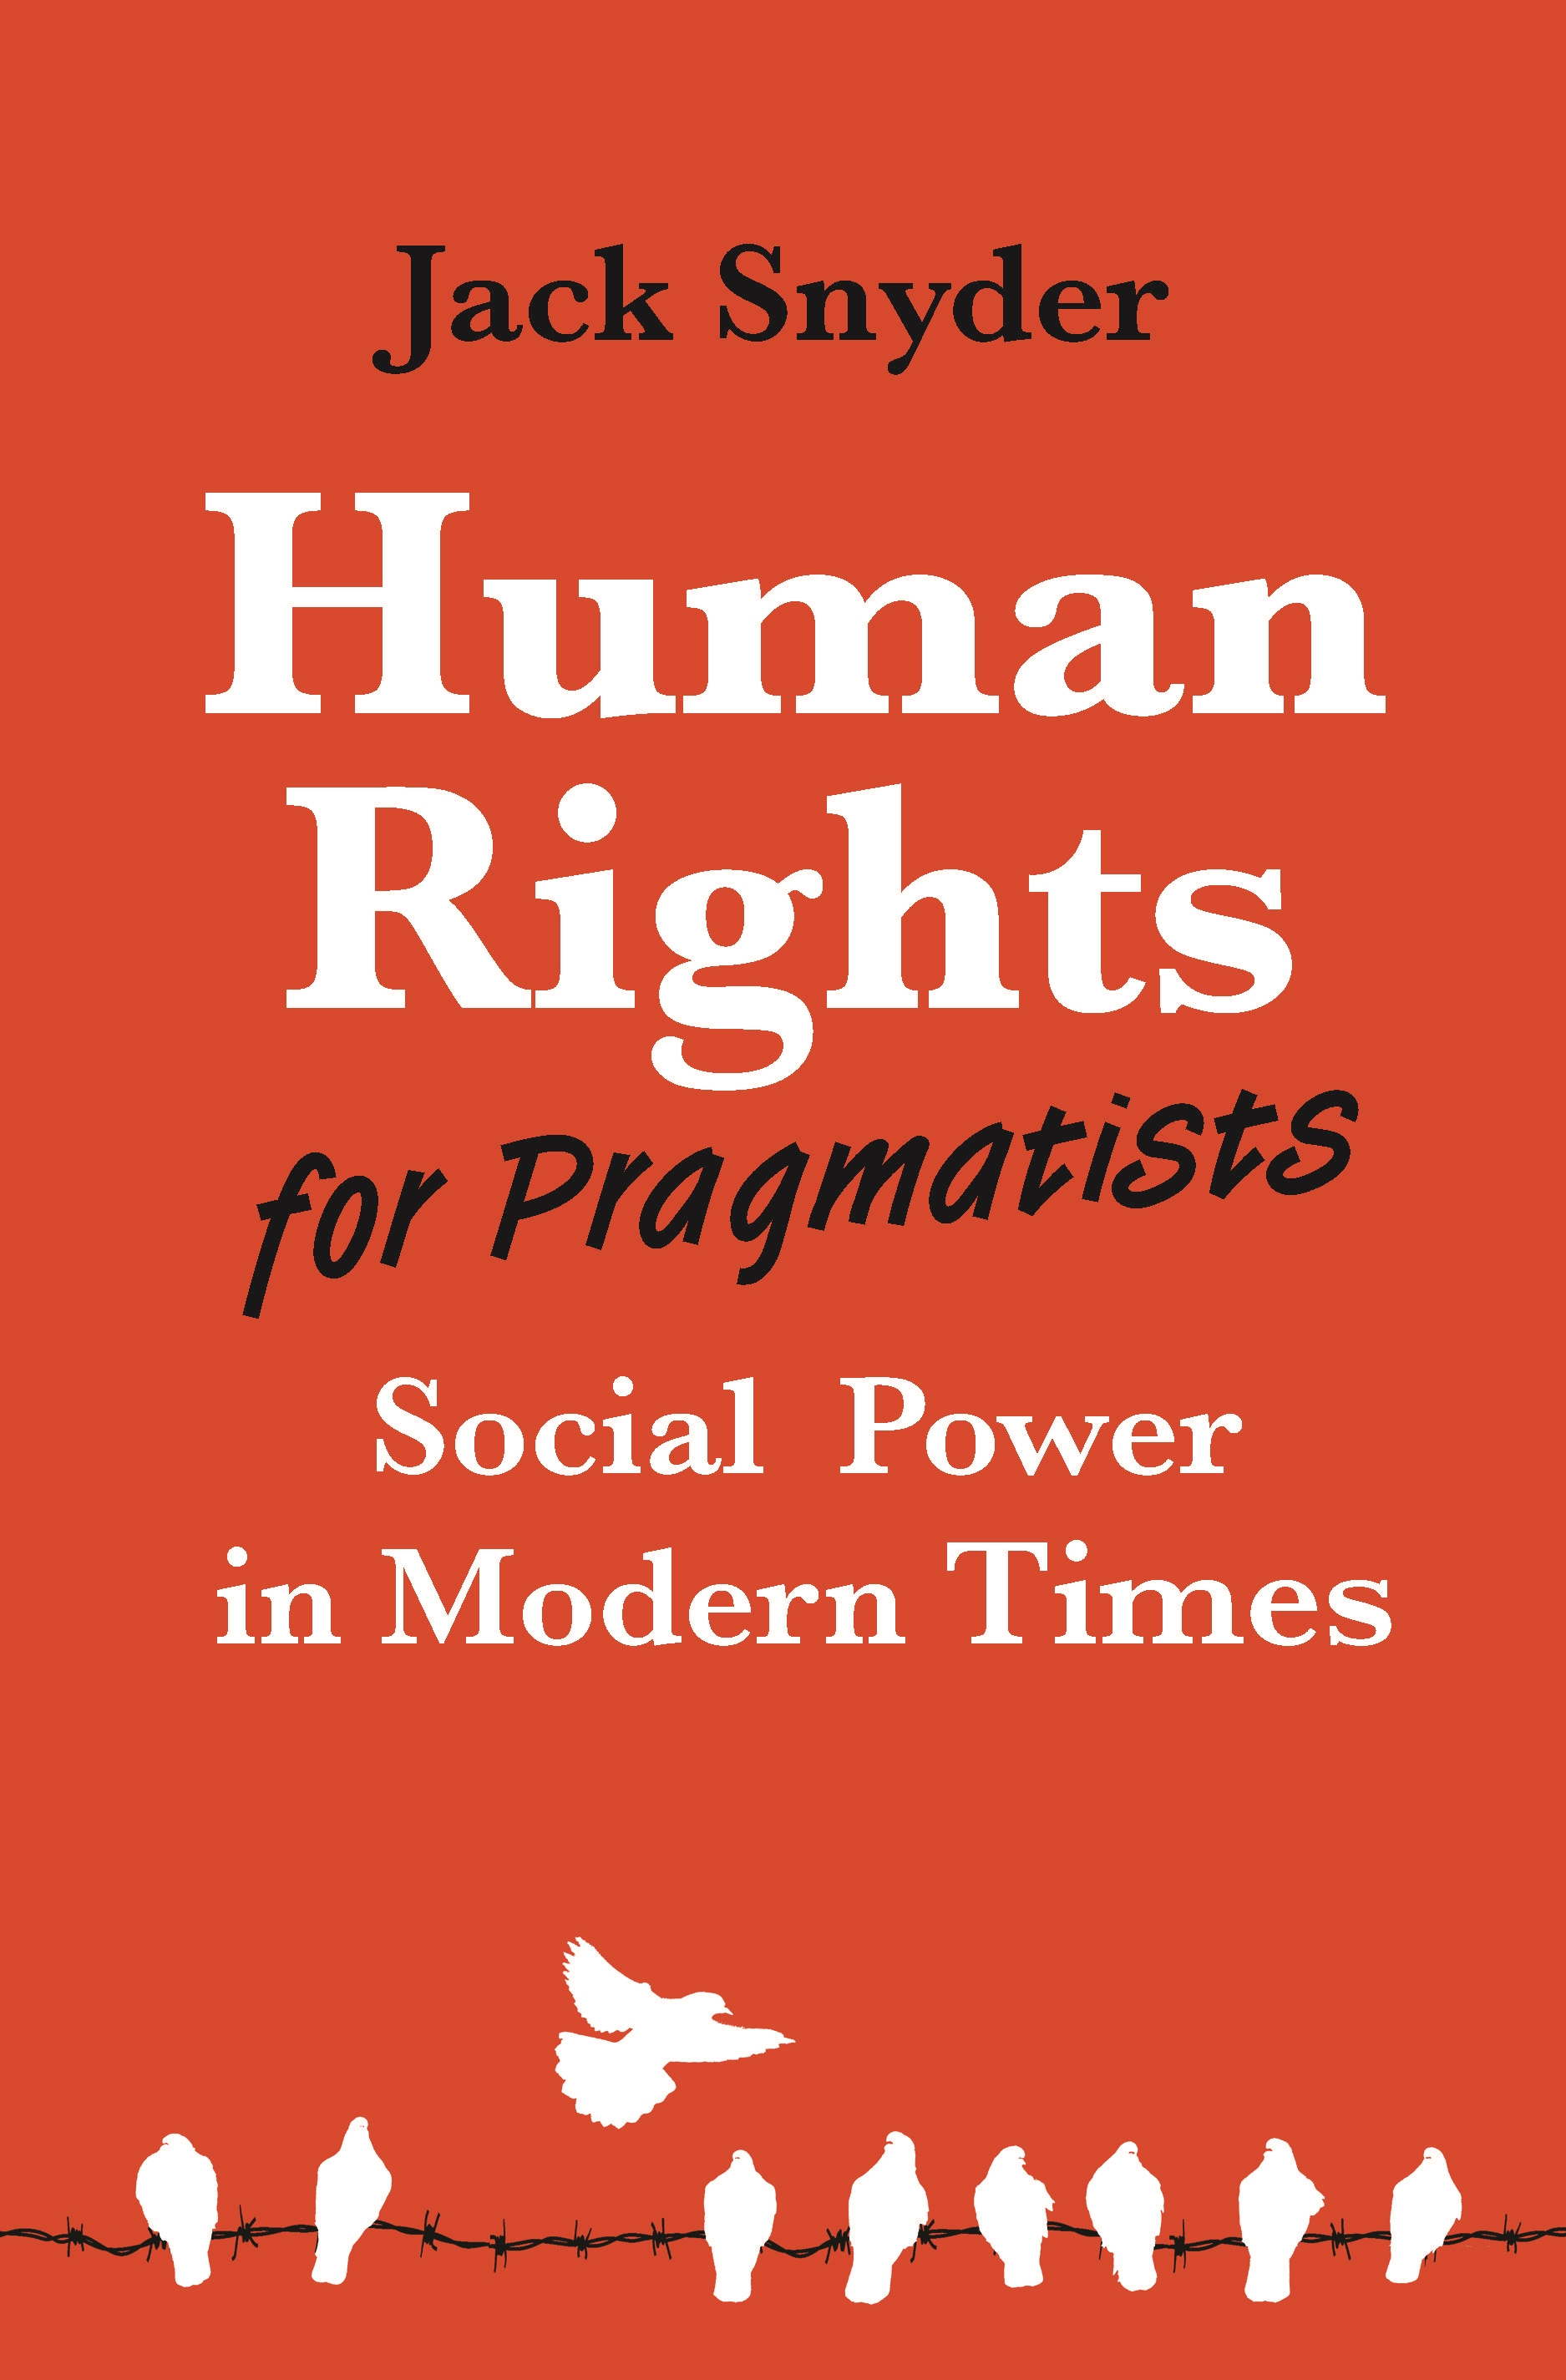
\includegraphics[width = .95\textwidth]{img/snyder2022}\\Jack Snyder (2022)
\end{minipage}

\end{frame}
% ----------------------------------------------------

% ----------------------------------------------------
\begin{frame}
\frametitle{Snyder's theses}
\centering

\begin{itemize}
  \item[1.] HR are \textit{beneficial} for modern economic production and governance
  \begin{itemize}
    \item vs. tradition based on favoritism and patronage
  \end{itemize}
  \item<2->[2.] HR prevail when the ruling coalition benefits from them
  \begin{itemize}
    \item if there is a winning coalition \textit{against} them, HR no longer in place
  \end{itemize}
  \item<3->[3.] The process depends on the creation of impartial institutions
  \begin{itemize}
    \item it doesn't work if HR are just norms that go unheeded
  \end{itemize}
  \item<4->[4.] Promotion as part of an ideology and culture
  \begin{itemize}
    \item vs. persuasion $\rightarrow$ institutionalization
  \end{itemize}
  \item<5->[5.] This is all a gradual process
  \begin{itemize}
    \item there are no short-cuts
  \end{itemize}
\end{itemize}

\end{frame}
% ----------------------------------------------------

% ----------------------------------------------------
\begin{frame}
\frametitle{Snyder's pragmatist approach}
\centering

\begin{itemize}
  \item Ideas about this argument?
  \item According to it, how can we promote human rights internationally? And what are the odds that we'll be successful?
  \item<2-> What does this mean for TJ policies?
\end{itemize}

\end{frame}
% ----------------------------------------------------

% ----------------------------------------------------
\begin{frame}
\frametitle{International norms and political change \scriptsize{(Finnemore \& Sikkink 1998)}}
\centering

\begin{itemize}
  \item Importance of \textit{norms} and the way they \textbf{change}
  \begin{itemize}
    \item Norms are not the opposite of strategic rationality
  \end{itemize}
  \item<2-> Examples of international norms:
  \begin{itemize}
    \item women's suffrage, laws of war, etc
  \end{itemize}
  \item<3-> How do wars emerge and evolve? Three phases
  \begin{itemize}
    \item[1.] Norm emergence (role of \textit{norm entrepreneurs})
    \item[2.] Norm cascade (\textit{imitation} dynamics)
    \item[3.] Internalization
  \end{itemize}
\end{itemize}

\end{frame}
% ----------------------------------------------------

% ----------------------------------------------------
\begin{frame}
\frametitle{The Justice Cascade}
\centering

\begin{minipage}{0.59\textwidth}\centering

\only<2->{
\begin{itemize}[<+->]
  \item Development of \BGyellow{HR accountability} norm at the international level
  \begin{itemize}
    \item individuals should be accountable to their actions in legal criminal courts
  \end{itemize}
  \item Individual criminal accountability\only<3->{, vs:}
  \begin{itemize}
    \item Amnesty
    \item State accountability
  \end{itemize}
  \item Spread of domestic, foreign, and international courts - and the legal backbone
  \item Role of \BGyellow{individual actors}: activists, lawyers, NGOs, etc
\end{itemize}}

\end{minipage}\hfill
\begin{minipage}{0.4\textwidth}\centering
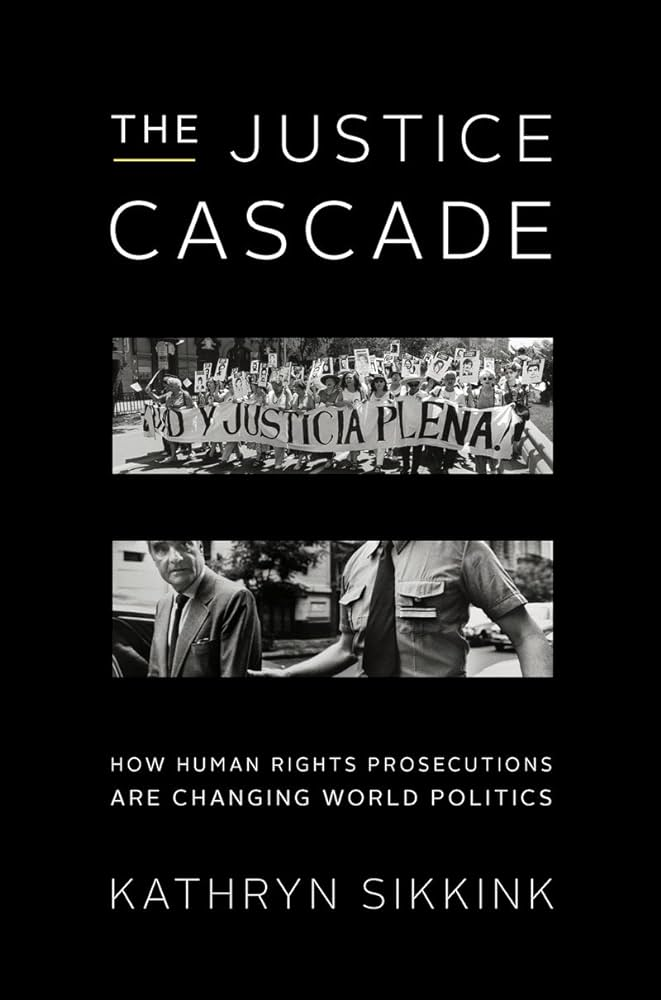
\includegraphics[width = \textwidth]{img/justice_cascade_book}\\Kathryn Sikkink (2011)
\end{minipage}

\end{frame}
% ----------------------------------------------------

% ----------------------------------------------------
\imageframe{img/justice_cascade}
% ----------------------------------------------------

% ----------------------------------------------------
\imageframe{img/sikkink_trials}
% ----------------------------------------------------

% ----------------------------------------------------
\imageframe{img/sikkink_by_region}
% ----------------------------------------------------

% ----------------------------------------------------
\againframe<4->{tj_q}
% ----------------------------------------------------


\end{document}
